\graphicspath{{introduction/fig/}}

\chapter{Introduction}
\label{chap:introduction}

\section{Background}
The majority of South Africa's public sector uses taxis as a means of transport. Millions of commuters use taxis frequently and depend on them for all of their mobility needs \cite{depttransport2023}.\\
Instead of using expensive and inconvenient formal public transportation like buses and trains, they offer an accessible and affordable substitute.
As a result, the effects of air quality in taxis on human health and the impact of taxi exhaust emissions are issues unique to South Africa.


%\cite{HACHEM2019133439}
%This citation is for air quality for drivers in traditional taxis cabs


\section{Problem Statement}
\section{Scope}
\section{Objectives}
\section{Report Overview}
%\section{}
%\section{}


%Chat GPT
%the impact of taxi exhaust emissions have become critical issues in South Africa. Studies have shown that the air quality at taxi ranks and inside taxis is often poor, exposing commuters, taxi drivers, and other road users to harmful pollutants. These pollutants can have serious health implications, including respiratory diseases, cardiovascular problems, and even cancer.

%Furthermore, the South African government has recognized the impact of taxi emissions on air quality and has taken steps to address the issue. In 2007, the government introduced regulations that required taxi operators to convert their vehicles to run on cleaner fuels, such as liquefied petroleum gas (LPG), compressed natural gas (CNG), or diesel with lower sulfur content. However, the implementation of these regulations has been slow and often ineffective, resulting in continued poor air quality in many areas.

%Therefore, there is a need for further research to assess the effectiveness of these regulations and to identify other potential solutions to improve cab air quality in South Africa. This thesis aims to address this need by investigating the air quality at taxi ranks and inside taxis in several major South African cities. The study will use air quality measurements to identify the types and levels of pollutants present in taxi emissions and assess their impact on human health. The findings will contribute to the development of evidence-based policies and strategies to reduce taxi emissions and improve air quality in South Africa, ultimately protecting the health of the country's citizens.







%This is some section with two table in it: Table~\ref{tbl:exemplars} and Table~\ref{tbl:abx_speaker}.

%	\begin{table}[!h]
%	    \mytable
%	    \caption{Performance of the unconstrained segmental Bayesian model on TIDigits1 over iterations in which the reference set is refined.}
%	    \begin{tabularx}{\linewidth}{@{}lCCCCC@{}}
%	        \toprule
%	        Metric     & 1 & 2 & 3 & 4 & 5 \\
%	        \midrule
%	        WER (\%)                        & $35.4$ & $23.5$ & $21.5$ & $21.2$ & $22.9$ \\
%	        Average cluster purity (\%)       & $86.5$ & $89.7$ & $89.2$ & $88.5$ & $86.6$ \\
%	        Word boundary $F$-score (\%)         & $70.6$ & $72.2$ & $71.8$ & $70.9$ & $69.4$ \\
%	        Clusters covering 90\% of data   & 20             & 13 & 13 & 13 & 13 \\
%	        \bottomrule
%	    \end{tabularx}
%	    \label{tbl:exemplars}
%	\end{table}


%\begin{table}[!h]
%    \renewcommand{\arraystretch}{1.1}
%    \centering
%    \caption{A table with an example of using multiple columns.}
%    \begin{tabularx}{0.65\linewidth}{@{}lCCr@{}}
%        \toprule
 %       & \multicolumn{2}{c}{Accuracy (\%)} \\
%        \cmidrule(lr){2-3}
%        Model    & Intermediate & Output & Bitrate\\
%        \midrule
%        Baseline & 27.5         & 26.4   & 116 \\
%        VQ-VAE   & 26.0         & 22.1   & 190 \\
%        CatVAE   & 28.7         & 24.3   & 215 \\
 %    \end{tabularx}
%    \label{tbl:abx_speaker}
%\end{table}

%\newpage

%This is a new page, showing what the page headings looks like, and showing how to refer to a figure like Figure~\ref{fig:cae_siamese}.

%\begin{figure}[!t]
%    \centering
%%     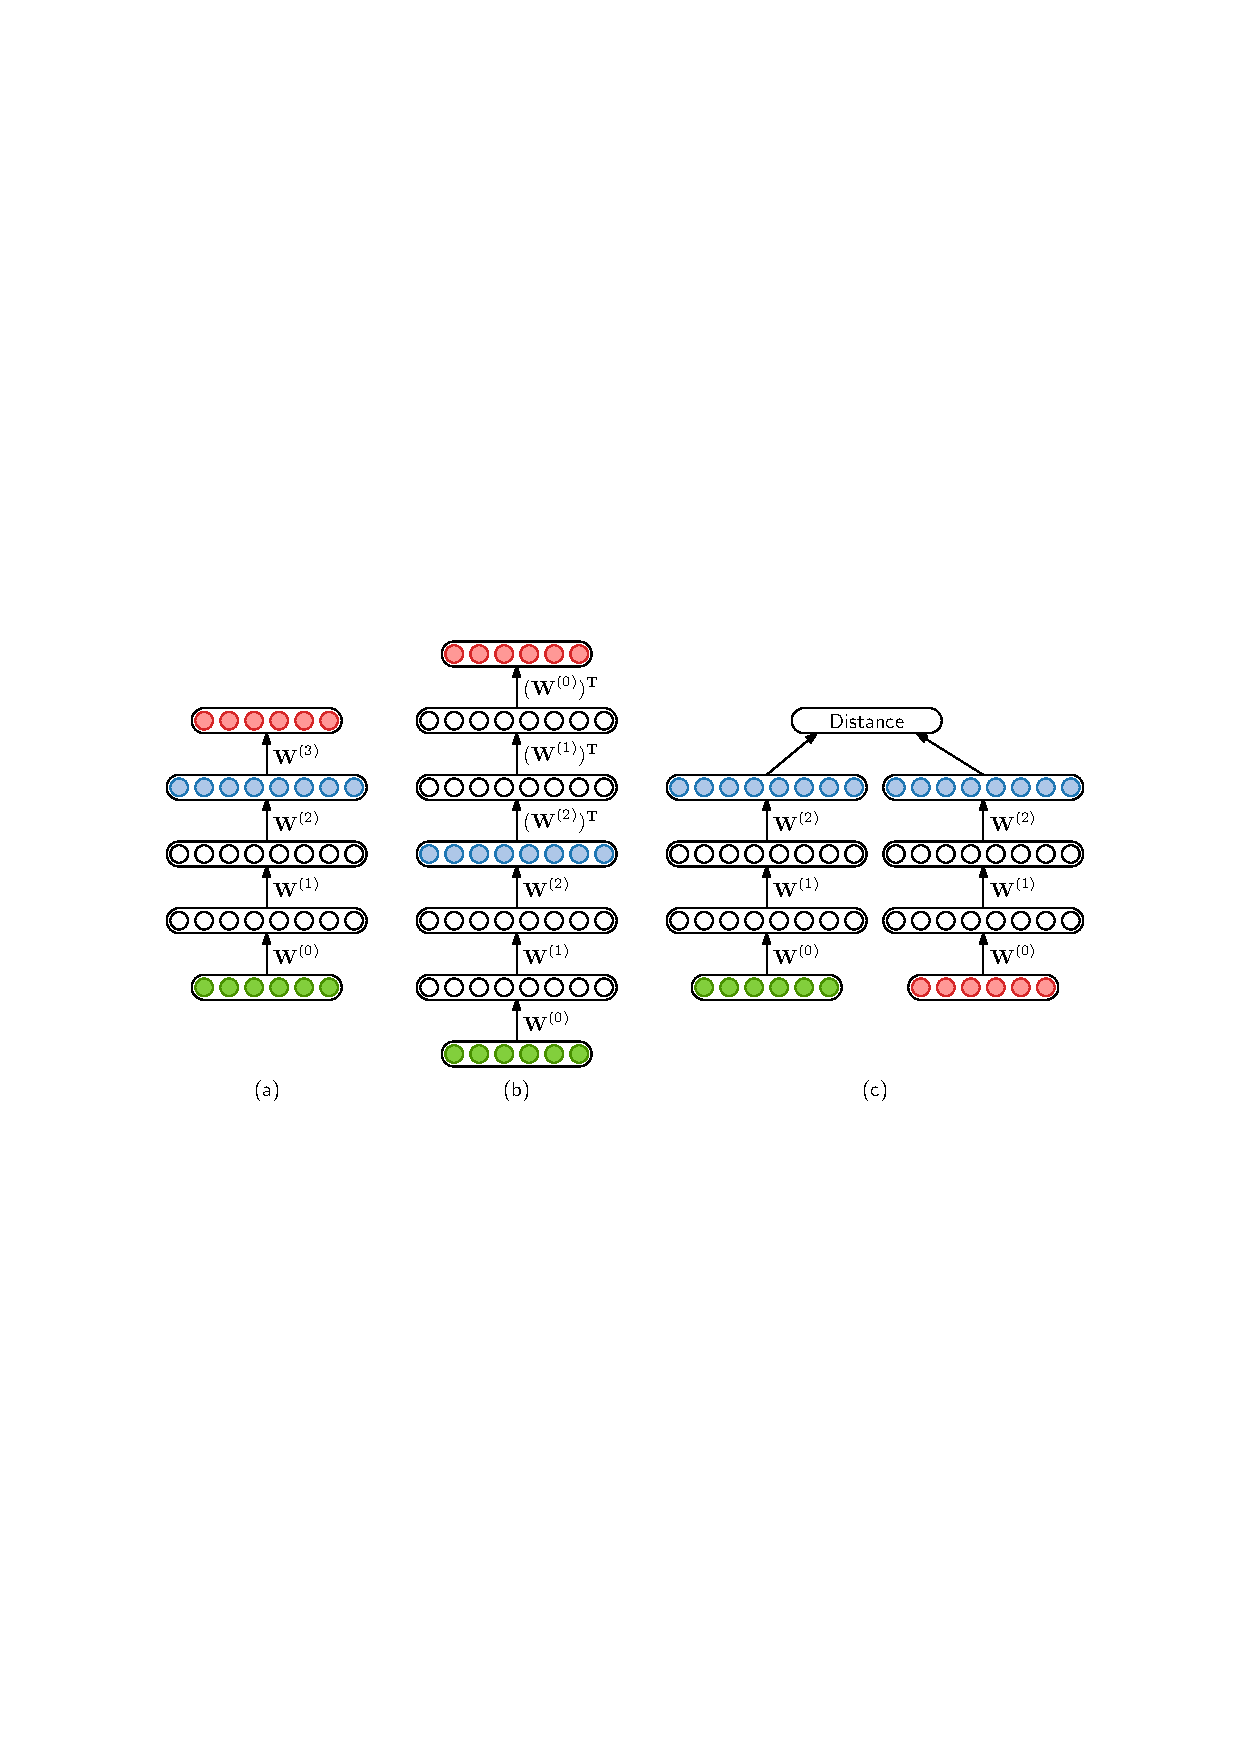
\includegraphics[width=\linewidth]{cae_siamese}
%    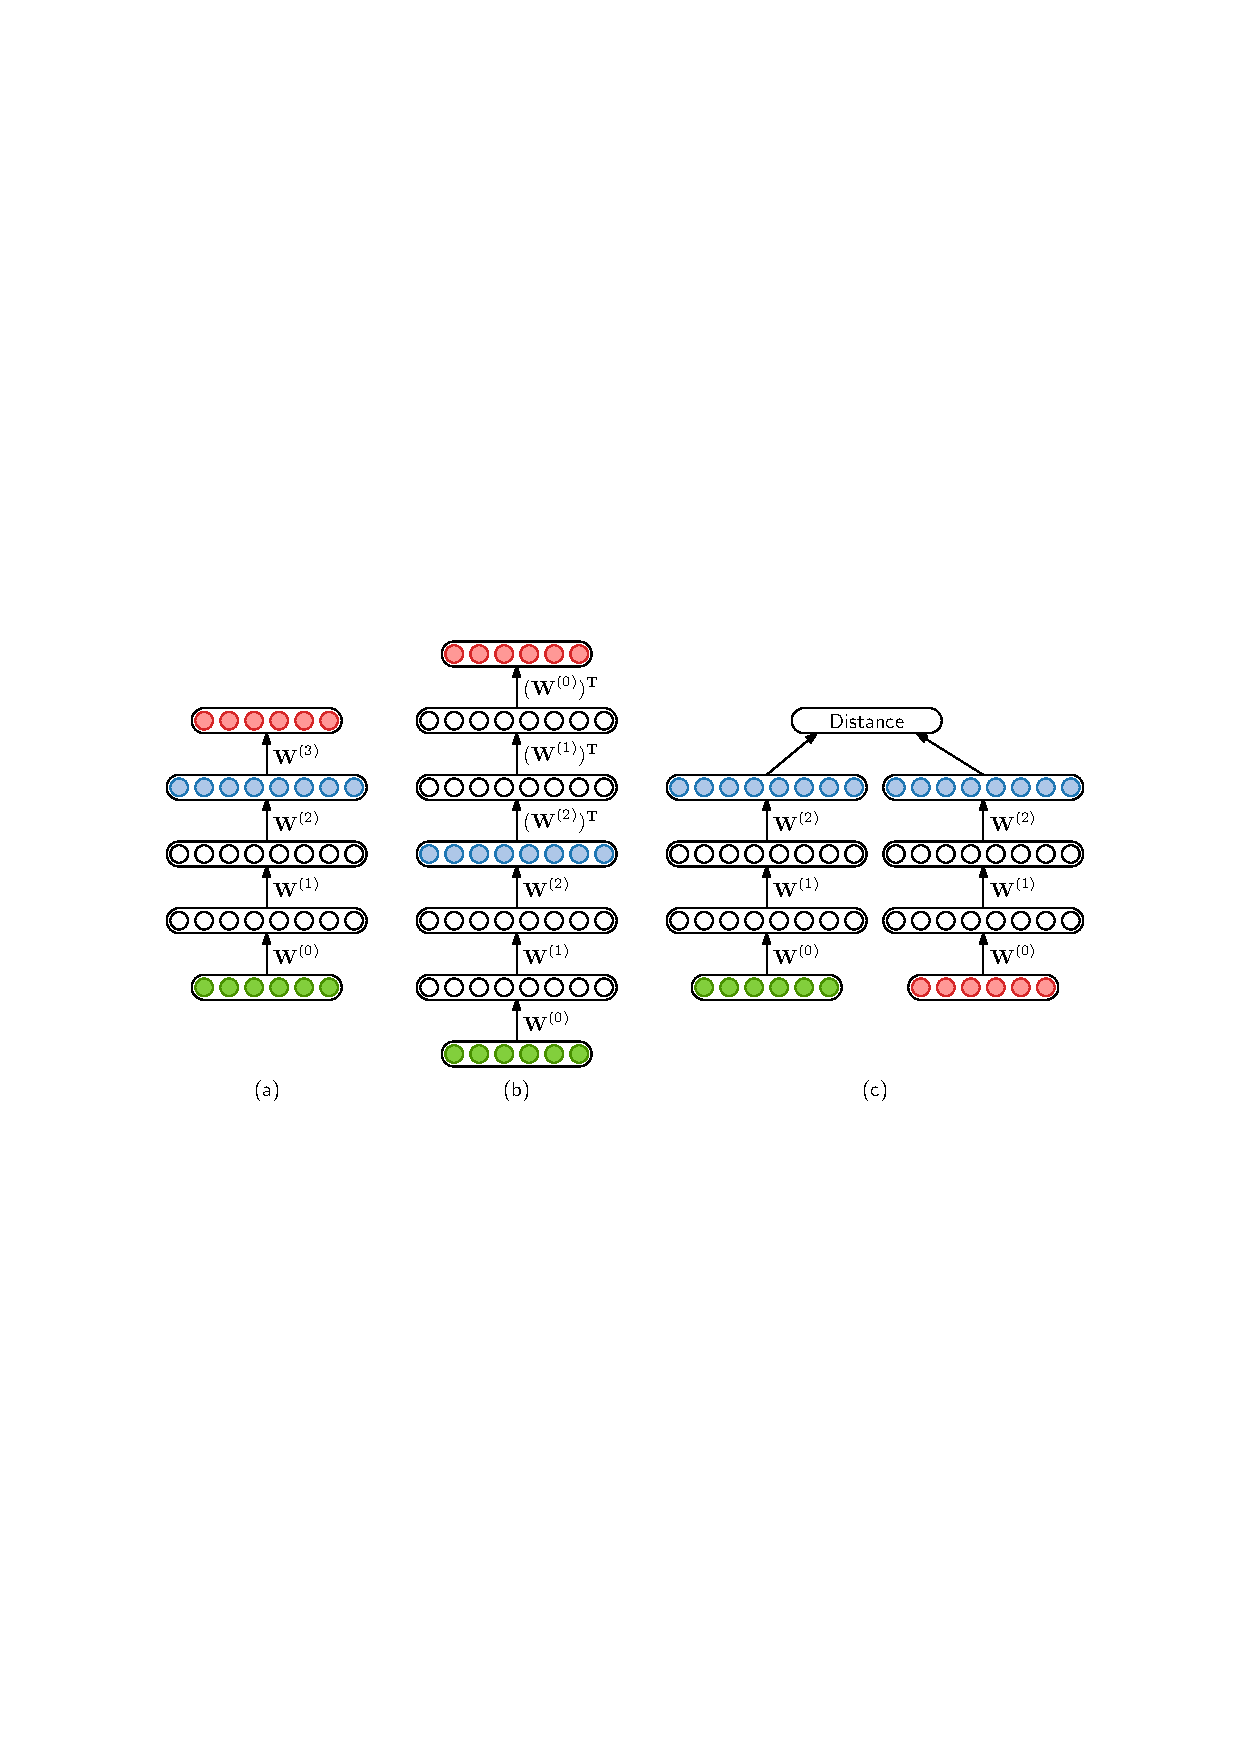
\includegraphics[width=0.918\linewidth]{cae_siamese}
%    \caption[I am the short caption that appears in the list of figures, without references.]{
%    (a) The cAE as used in this chapter. The encoding layer (blue) is chosen based on performance on a development set.
%    (b) The cAE with symmetrical tied weights. The encoding from the middle layer (blue) is always used.
%    (c) The siamese DNN. The cosine distance between aligned frames (green and red) is either minimized or maximized depending on whether the frames belong to the same (discovered) word or not.
%    A cAE can be seen as a type of DNN.
%    }
%    \label{fig:cae_siamese}
%\end{figure}

%
%The following is an example of an equation:
%\begin{equation}
%P(\vec{z} | \vec{\alpha}) = \int_{\vec{\pi}} P(\vec{z} | \vec{\pi}) \, p(\vec{\pi} | \vec{\alpha}) \, \textrm{d} \vec{\pi}
%= \int_{\vec{\pi}} \prod_{k = 1}^K \pi_k^{N_k} \frac{1}{B(\vec{\alpha})} \prod_{k = 1}^K \pi_k^{\alpha_k - 1} \, \textrm{d} \vec{\pi}
%\label{eq:example_equation}
%\end{equation}
%which you can subsequently refer to as~\eqref{eq:example_equation} or Equation~\ref{eq:example_equation}.
%But make sure to consistently use the one or the other (and not mix the two ways of referring to equations).